%=========================================================
% MODULE 2 : PROCESS IN MODEL DEVELOPMENT AND VERSIONING
% Textbook 1: Part II (Chapter 4 - Developing Models)
% Mark Treveil et al., Introducing MLOps, O'Reilly, 2020
%=========================================================

%=========================================================
\section{Module 2: Developing Models}
%=========================================================

\begin{frame}{Developing Models}
\begin{enumerate}
\item<1-> Anyone serious about MLOps needs at least a \textbf{cursory understanding} of the model development process.
\item<2-> Model development is one element of the \textbf{larger ML project life cycle}.
\item<3-> Depending on the situation, it ranges from \textbf{quite simple} to \textbf{extremely complex}.
\item<4-> It \textbf{dictates the constraints} of subsequent usage, monitoring, and maintenance of models.
\item<5-> This module covers model development \textbf{in the context of MLOps}: building models so that MLOps considerations are easier to implement later.
\end{enumerate}
\end{frame}

%---------------------------------------------------------
\begin{frame}{Model Development in the ML Project Life Cycle}
\begin{figure}
\centering
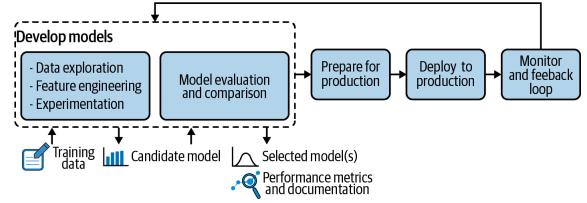
\includegraphics[width=0.66\linewidth]{images/Fig4_1_model_development.png}
\caption{Model development highlighted in the larger context of the ML project life cycle}
\end{figure}
\vspace{-0.3cm}
\begin{enumerate}\small
\item<1-> \textbf{Develop models:} Data exploration, feature engineering, experimentation, followed by model evaluation and comparison.
\item<2-> \textbf{Inputs/outputs:} Training data goes in; candidate models are produced; selected model(s) come out with performance metrics and documentation.
\item<3-> Selected models flow to \textbf{prepare for production} $\rightarrow$ \textbf{deploy to production} $\rightarrow$ \textbf{monitor and feedback loop}, which loops back to development.
\end{enumerate}
\end{frame}

%---------------------------------------------------------
\begin{frame}{Implications of Development Choices}
\begin{enumerate}
\item<1-> The implications of the \textbf{data collection process} are straightforward: a model can easily become \textbf{stale}.
\item<2-> For other parts of the model, the effects may be \textbf{less obvious}.
\item<3-> \textbf{Feature creation example:} Feeding a \textbf{date} versus a flag for \textbf{public holiday} can change performance, and also imposes different constraints on updating the model.
\item<4-> \textbf{Metrics example:} The metrics used for evaluating and comparing models may enable \textbf{automatic switching} to the best version later.
\end{enumerate}
\end{frame}

%=========================================================
\subsection{What Is a Machine Learning Model?}
%=========================================================

\begin{frame}{What Is a Machine Learning Model? --- In Theory}
\begin{enumerate}
\item<1-> An ML model is a \textbf{projection of reality}: a partial and approximate representation of some aspects of a real thing or process.
\item<2-> Once trained, it boils down to a \textbf{mathematical formula} that yields a result (a probability or a raw value) when fed inputs.
\item<3-> Models are based on \textbf{statistical theory}; ML algorithms are the \textbf{tools that build models} from training data.
\item<4-> Training data represents the world \textbf{as it was at collection time}.
\item<5-> Hence models can predict well \textbf{when the future looks like the past}.
\end{enumerate}
\end{frame}

%---------------------------------------------------------
\begin{frame}{Generalization Capacity and Examples}
\begin{enumerate}
\item<1-> \textbf{Generalization capacity:} The ability to predict accurately for cases not exactly like the input data.
\item<2-> Even outputs like \textbf{horses with zebra stripes} (CycleGAN) come from modeling a probability distribution.
\item<3-> \textbf{House price example:}
    \begin{itemize}
    \item Inputs: surface area, bedrooms, bathrooms, year of construction, location.
    \item Contextual inputs: housing market state, seller urgency.
    \item With enough historical data and stable market conditions, a reasonable estimate is possible.
    \end{itemize}
\item<4-> \textbf{Health example:} Classification models predict the \textbf{probability} of developing a disease, sometimes with a \textbf{confidence interval}.
\end{enumerate}
\end{frame}

%---------------------------------------------------------
\begin{frame}{What Is a Machine Learning Model? --- In Practice}
\begin{enumerate}
\item<1-> A model is the \textbf{set of parameters} necessary to rebuild and apply the formula.
\item<2-> It is usually \textbf{stateless and deterministic}: the same inputs give the same outputs (exception: online learning).
\item<3-> It includes \textbf{all transformations} from input data to the final formula, plus derived data (classification or decision).
\item<4-> In practice, whether ML-based or not, a model is \textbf{a computable mathematical function} applied to input data, one row at a time.
\item<5-> \textbf{House price example:} Zip codes may be replaced by derived inputs (average income, population density, amenities); this transformation is \textbf{part of the model}.
\end{enumerate}
\end{frame}

%---------------------------------------------------------
\begin{frame}{Richer Model Outputs and Packaging}
\begin{enumerate}
\item<1-> Outputs can be \textbf{richer than a single number}.
\item<2-> \textbf{Fraud detection:} Outputs a probability (maybe with a confidence interval); a \textbf{fine-tuned threshold} decides fraud classification based on costs.
\item<3-> Some models include \textbf{recommendations or decisions}: which product to show, which treatment gives the most probable recovery.
\item<4-> All transformations and associated data are part of the model, but are \textbf{not always bundled} as a single artifact.
\item<5-> Different parts have \textbf{varying constraints} (different refresh rates, external sources, etc.).
\end{enumerate}
\end{frame}

%=========================================================
\subsection{Required Components}
%=========================================================

\begin{frame}{Required Components of an ML Model (Table 4-1)}
\begin{table}
\centering
\renewcommand{\arraystretch}{1.2}
\scriptsize
\begin{tabular}{|p{2.6cm}|p{11cm}|}
\hline
\textbf{ML Component} & \textbf{Description} \\ \hline
Training data & Usually labeled with examples of what is modeled (supervised learning). Must be good data --- e.g., WWII damaged-plane data suffered from \textbf{survivor bias}. \\ \hline
Performance metric & What the model seeks to optimize; chosen carefully to avoid the \textbf{cobra effect}. If 95\% of data is class A, raw accuracy rewards always predicting A. \\ \hline
ML algorithm & Models work in various ways with pros and cons; selection depends on priorities: performance, stability, interpretability, computation cost. \\ \hline
Hyperparameters & Configurations for ML algorithms: the ways the algorithm goes to find its parameters. E.g., \textbf{depth} of a decision tree. \\ \hline
Evaluation dataset & Data different from the training set, used to evaluate performance on unseen data (\textbf{generalization}). \\ \hline
\end{tabular}
\end{table}
\begin{enumerate}\small
\item<1-> The number and complexity of these components makes good MLOps \textbf{challenging}.
\item<2-> \textbf{Algorithm choice} is yet another piece of the puzzle.
\end{enumerate}
\end{frame}

%---------------------------------------------------------
\begin{frame}{Required Components --- Explained}
\begin{enumerate}
\item<1-> \textbf{Training data:} Quality and representativeness decide model quality; biased samples (survivor bias) lead to wrong conclusions.
\item<2-> \textbf{Performance metric:} Defines ``good''; a poorly chosen metric produces unintended behavior (cobra effect).
\item<3-> \textbf{ML algorithm:} Contains the basic formula; must suit the task and priorities.
\item<4-> \textbf{Parameters vs hyperparameters:} Parameters are \textbf{learned} operations/operands of the formula; hyperparameters \textbf{guide how} they are found.
\item<5-> \textbf{Evaluation dataset:} Separate from training data to measure generalization.
\end{enumerate}
\end{frame}

%=========================================================
\subsection{Different ML Algorithms, Different MLOps Challenges}
%=========================================================

\begin{frame}{MLOps Considerations by Algorithm Type (Table 4-2)}
\begin{table}
\centering
\renewcommand{\arraystretch}{1.2}
\scriptsize
\begin{tabular}{|p{2cm}|p{2.4cm}|p{9.4cm}|}
\hline
\textbf{Algorithm Type} & \textbf{Name} & \textbf{MLOps Considerations} \\ \hline
\multirow{2}{*}{Linear} & Linear regression & Tendency for overfitting. \\ \cline{2-3}
 & Logistic regression & Tendency for overfitting. \\ \hline
\multirow{3}{*}{Tree-based} & Decision tree & Can be unstable --- small data changes can greatly change the tree structure. \\ \cline{2-3}
 & Random forest & Predictions difficult to understand (Responsible AI challenge); relatively slow to output predictions. \\ \cline{2-3}
 & Gradient boosting & Predictions difficult to understand; small changes in features or training set can radically change the model. \\ \hline
Deep learning & Neural networks & Almost impossible to interpret; extremely slow to train; need a lot of power and data. Would a simpler model work just as well? \\ \hline
\end{tabular}
\end{table}
\begin{enumerate}\small
\item<1-> All algorithms model patterns in past data; they differ in characteristics and \textbf{MLOps challenges}.
\item<2-> Quality and relevance of past experience are the \textbf{key factors} in effectiveness.
\end{enumerate}
\end{frame}

%---------------------------------------------------------
\begin{frame}{Algorithm Choice: Governance and Computing Power}
\begin{enumerate}
\item<1-> \textbf{Governance} may drive algorithm choice: regulated environments needing explanations (financial services) avoid opaque models like neural networks and favor \textbf{decision trees}.
\item<2-> Often the trade-off is on \textbf{cost}, not performance: simpler techniques need more costly \textbf{manual feature engineering}.
\item<3-> \textbf{Computing power:} ML development is \textbf{inversely proportional} to the cost of computing power.
\item<4-> New algorithms arose as compute became available; random forest and gradient boosting were expensive 20 years ago.
\item<5-> They brought \textbf{ease of use}, lowering development cost and enabling new use cases.
\item<6-> Most algorithms still operate with \textbf{all training data in memory}, not distributed big data.
\end{enumerate}
\end{frame}

%=========================================================
\subsection{Data Exploration}
%=========================================================

\begin{frame}{Data Exploration}
\begin{enumerate}
\item<1-> Data scientists must first grasp \textbf{what the data looks like}; a model is only as good as its training data.
\item<2-> Issues: \textbf{incompleteness, inaccuracy, inconsistency}.
\item<3-> Exploration processes include:
    \begin{itemize}
    \item Documenting how data was collected and assumptions made.
    \item Summary statistics: column domains, missing values, mistakes, outliers.
    \item Examining data distributions.
    \item Cleaning, filling, reshaping, filtering, clipping, sampling.
    \item Checking correlations, statistical tests on subpopulations, fitting distributions.
    \item Comparing with other data or literature.
    \end{itemize}
\item<4-> \textbf{Domain knowledge} is essential, e.g., industrial sensor data needs equipment expertise to spot abnormal outliers.
\end{enumerate}
\end{frame}

%=========================================================
\subsection{Feature Engineering and Selection}
%=========================================================

\begin{frame}{Feature Engineering and Selection}
\begin{enumerate}
\item<1-> \textbf{Features} are how data is presented to a model, informing it on things it may not infer by itself.
\end{enumerate}
\begin{table}
\centering
\renewcommand{\arraystretch}{1.2}
\scriptsize
\begin{tabular}{|p{2.5cm}|p{10.5cm}|}
\hline
\textbf{Category} & \textbf{Description} \\ \hline
Derivatives & Infer new information from existing information --- e.g., what day of the week is this date? \\ \hline
Enrichment & Add new external information --- e.g., is this day a public holiday? \\ \hline
Encoding & Present the same information differently --- e.g., day of week or weekday versus weekend. \\ \hline
Combination & Link features together --- e.g., backlog size weighted by the complexity of its items. \\ \hline
\end{tabular}
\end{table}
\begin{enumerate}\setcounter{enumi}{1}
\item<2-> \textbf{Process duration example:} From a date, derive day of week or distance to the next public holiday; consider location-specific business calendars.
\item<3-> \textbf{House price example:} Use average income and population density instead of zip code to generalize better.
\end{enumerate}
\end{frame}

%---------------------------------------------------------
\begin{frame}{Feature Engineering Techniques}
\begin{enumerate}
\item<1-> A market exists for \textbf{complementary data} beyond open data; enrichment services save time and effort.
\item<2-> \textbf{Impact coding:} Replace a modality by the \textbf{average target value} for that modality (at some information loss).
\item<3-> Most algorithms require a \textbf{table of numbers}: each row a sample, all from the same dataset.
\item<4-> \textbf{One-hot encoding:} A feature with values Raspberry, Blueberry, Strawberry becomes three yes/no features.
\item<5-> \textbf{Embeddings:} Deep learning transforms text and images into tables of numbers, enabling \textbf{transfer learning}.
\end{enumerate}
\end{frame}

%---------------------------------------------------------
\begin{frame}{Transfer Learning}
\begin{block}{Transfer Learning}
The technique of using information gained from solving one problem in solving a different problem.
\end{block}
\vspace{0.2cm}
\begin{enumerate}
\item<1-> Significantly \textbf{accelerates learning} of second or subsequent tasks.
\item<2-> Very popular in \textbf{deep learning}, where training resources can be enormous.
\item<3-> \textbf{Example:} A model trained on images without forks may still give a useful embedding for a fork detector, since it learned to detect similar \textbf{human-made objects}.
\end{enumerate}
\end{frame}

%---------------------------------------------------------
\begin{frame}{How Feature Selection Impacts MLOps Strategy}
\begin{enumerate}
\item<1-> More features may give more accuracy, more fairness, or compensate for missing information.
\item<2-> \textbf{Downsides} affecting MLOps:
    \begin{itemize}
    \item The model becomes more \textbf{expensive to compute}.
    \item More features need more inputs and \textbf{more maintenance}.
    \item Some loss of \textbf{stability}.
    \item The number of features can raise \textbf{privacy concerns}.
    \end{itemize}
\item<3-> \textbf{Automated feature selection} uses heuristics: correlation with the target, or training a simple model on a subset to find the strongest predictors.
\item<4-> Tools like \textbf{Auto-sklearn} or AutoML cross-reference features against the target to keep the most useful ones.
\end{enumerate}
\end{frame}

%---------------------------------------------------------
\begin{frame}{Human Choices and Feature Stores}
\begin{enumerate}
\item<1-> Some choices need \textbf{human intervention}, e.g., collecting additional information.
\item<2-> \textbf{Business-friendly features} improve performance, ease adoption, simplify explanations, and reduce \textbf{modeling debt}.
\item<3-> Trade-offs exist between time spent understanding the model, expected value, and risk.
\item<4-> \textbf{Feature stores:} Central repositories of features for business entities, created once and \textbf{reused}.
\item<5-> They combine an \textbf{offline} part (slower, more powerful) and an \textbf{online} part (fast, real-time), kept consistent.
\item<6-> ML is often the ``\textbf{high-interest credit card of technical debt}''; feature stores are one way to reverse this.
\end{enumerate}
\end{frame}

%=========================================================
\subsection{Experimentation}
%=========================================================

\begin{frame}{Experimentation}
\begin{enumerate}
\item<1-> Experimentation occurs \textbf{throughout} model development; important decisions are justified by experiments or research.
\item<2-> It can take many shapes: full predictive models, statistical tests, charting data.
\item<3-> \textbf{Goals of experimentation:}
    \begin{itemize}
    \item Assess how useful a model can be built given the Table 4-1 components.
    \item Find the best modeling parameters (algorithms, hyperparameters, preprocessing).
    \item Tune the \textbf{bias/variance trade-off} for a given training cost.
    \item Balance model improvement against computation cost --- how good is \textbf{good enough}?
    \end{itemize}
\end{enumerate}
\end{frame}

%---------------------------------------------------------
\begin{frame}{Bias and Variance}
\begin{enumerate}
\item<1-> \textbf{High bias (underfitting):} Fails to discover rules that could be learned from training data, due to reductive assumptions making it \textbf{overly simplistic}.
\item<2-> \textbf{High variance (overfitting):} Sees patterns in noise and predicts every variation, becoming complex and \textbf{not generalizing} beyond training data.
\item<3-> Experimentation aims to find the right balance between the two for the problem at hand.
\end{enumerate}
\end{frame}

%---------------------------------------------------------
\begin{frame}{Experimentation Tools and Budget}
\begin{enumerate}
\item<1-> Tools test possibilities \textbf{semiautomatically}: define the search space from prior knowledge and constraints (computation, budget).
\item<2-> \textbf{Stratified modeling:} Train one model per store (e.g., demand forecasting) instead of one model for all stores.
\item<3-> Trying all combinations becomes \textbf{intractable}; define a \textbf{time/computation budget} and an acceptability threshold.
\item<4-> The process may need repeating whenever data or problem constraints \textbf{change significantly}.
\item<5-> All experiments, assumptions, and conclusions may need to be \textbf{rerun and reexamined}.
\item<6-> Platforms automate workflows, preserve processing for repeatability, and support \textbf{version control and experimental branching}.
\end{enumerate}
\end{frame}

%=========================================================
\subsection{Evaluating and Comparing Models}
%=========================================================

\begin{frame}{Evaluating and Comparing Models}
\begin{enumerate}
\item<1-> George E. P. Box: \textbf{all models are wrong, but some are useful}.
\item<2-> A model should be ``\textbf{good enough to be useful}'' while avoiding the \textbf{uncanny valley} (good overall, catastrophic for a subset such as an underrepresented population).
\item<3-> Evaluate in context and \textbf{compare with what existed before} (previous model or rules-based process).
\item<4-> A disappointing absolute performance can still help, e.g., a slightly better demand forecast may give \textbf{huge cost savings}.
\item<5-> A \textbf{perfect score is suspicious}: it may indicate \textbf{data leakage} or \textbf{overfitting}.
\end{enumerate}
\end{frame}

%---------------------------------------------------------
\begin{frame}{Choosing Evaluation Metrics}
\begin{enumerate}
\item<1-> The metric chosen can lead to \textbf{very different models} (cobra effect).
\item<2-> \textbf{Accuracy} is rarely the best fit for \textbf{unbalanced classes}.
\item<3-> \textbf{Example:} If the positive class occurs 5\% of the time, always predicting negative gives 95\% accuracy but is \textbf{utterly useless}.
\item<4-> There is \textbf{no one-size-fits-all} metric.
\item<5-> Understand the metric's limits and trade-offs (\textbf{mathematics side}) and its impact on optimization (\textbf{business side}).
\end{enumerate}
\end{frame}

%---------------------------------------------------------
\begin{frame}{Cross-Testing and Cross-Validation}
\begin{enumerate}
\item<1-> \textbf{Cross-testing:} Evaluate the metric on a \textbf{holdout dataset} not used for training.
\item<2-> Data can be held out at multiple steps (metric evaluation, hyperparameter optimization).
\item<3-> \textbf{k-fold cross-validation:} Rotate held-out parts to train and evaluate multiple times; costs training time but shows \textbf{metric stability}.
\item<4-> The holdout set can be the \textbf{most recent records}, giving more realistic estimates for future predictions.
\item<5-> Recent-data holdout also helps assess whether data \textbf{drifted} between training and holdout.
\end{enumerate}
\end{frame}

%---------------------------------------------------------
\begin{frame}{Dataset Split for Model Evaluation}
\begin{columns}[T]
\begin{column}{0.50\textwidth}
\begin{figure}
\centering
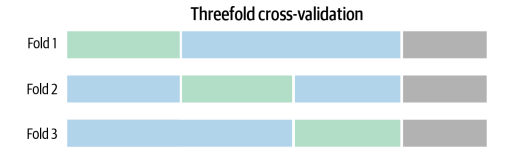
\includegraphics[width=\linewidth]{images/Fig4_2_cross_validation.png}
\caption{An example of dataset split for model evaluation}
\end{figure}
\end{column}
\begin{column}{0.48\textwidth}
\begin{enumerate}\small
\item<1-> \textbf{Gray} block: The \textbf{test (holdout) dataset}, set aside for final evaluation.
\item<2-> The remaining data is split into \textbf{three parts} (threefold cross-validation).
\item<3-> For each hyperparameter combination, the model is trained on the \textbf{blue} parts and validated on the \textbf{green} part --- three times.
\item<4-> Blue/green datasets are used with \textbf{all} combinations.
\item<5-> The gray dataset is used \textbf{only once}, with the best hyperparameter combination.
\end{enumerate}
\end{column}
\end{columns}
\end{frame}

%---------------------------------------------------------
\begin{frame}{Comparing Retrained Models}
\begin{enumerate}
\item<1-> Models are often \textbf{periodically retrained} with the same algorithms, hyperparameters, and features on more recent data.
\item<2-> Next, \textbf{compare} the new version against the previous one.
\item<3-> Also verify that \textbf{previous assumptions still hold}:
    \begin{itemize}
    \item The problem has not fundamentally shifted.
    \item Earlier modeling choices still fit the data.
    \end{itemize}
\item<4-> This is part of \textbf{performance and drift monitoring} (Chapter 7).
\end{enumerate}
\end{frame}

%---------------------------------------------------------
\begin{frame}{Cross-Checking Model Behavior}
\begin{enumerate}
\item<1-> Beyond raw metrics, understand \textbf{how the model behaves}, in proportion to its impact.
\item<2-> Ensure the model is not \textbf{actively harmful}: predicting that all patients need a doctor scores high on prevention but fails resource allocation.
\item<3-> \textbf{Reasonable steps:}
    \begin{itemize}
    \item Cross-check \textbf{different metrics}, not only the optimized one.
    \item Check reactions to different inputs (plot average prediction vs. input values).
    \item Compare behavior across \textbf{subpopulations} (e.g., error rate for males vs. females).
    \end{itemize}
\item<4-> These analyses show \textbf{correlation, not causality}; use with care for what-if analysis on unseen values.
\item<5-> Comparisons need the \textbf{full environment} (tooling, data): same settings/different data for drift, same data/different settings for performance.
\end{enumerate}
\end{frame}

%=========================================================
\subsection{Impact of Responsible AI on Modeling}
%=========================================================

\begin{frame}{Impact of Responsible AI on Modeling}
\begin{enumerate}
\item<1-> Individual predictions may need to be \textbf{explainable}: which features pushed the prediction one way or another.
\item<2-> \textbf{Shapley value:} Average marginal contribution of a feature value across all possible coalitions.
\item<3-> \textbf{Individual Conditional Expectation (ICE):} Shows the dependence between the target function and features of interest.
\item<4-> \textbf{Example:} A hormone level may indicate a health issue in general, but for a \textbf{pregnant woman} it indicates no risk.
\item<5-> Some legal frameworks mandate explainability for decisions affecting humans (e.g., \textbf{loan denial}).
\end{enumerate}
\end{frame}

%---------------------------------------------------------
\begin{frame}{Dimensions of Explainability}
\begin{enumerate}
\item<1-> Deep learning networks are called \textbf{black-box models} due to complexity.
\item<2-> Their formula is conceptually simple but \textbf{very large}, impossible to apprehend intuitively.
\item<3-> Global and local tools (partial dependence plots, Shapley values) give \textbf{insights}, but do not make the model intuitive.
\item<4-> Communicating a rigorous, intuitive understanding requires \textbf{limiting model complexity}.
\item<5-> \textbf{Fairness requirements} can also impose dimensioning constraints on model development.
\end{enumerate}
\end{frame}

%---------------------------------------------------------
\begin{frame}{Fairness Example: Weequay and Togruta}
\begin{enumerate}
\item<1-> A US-based organization trains a model to predict worker performance and hires based on it.
\item<2-> Hypothetically, everyone belongs to one of two groups: \textbf{Weequay} or \textbf{Togruta}.
\item<3-> More Weequay attend university, so Weequay applicants are \textbf{more numerous and more qualified}.
\item<4-> \textbf{Equal opportunity:} Hiring should not depend on group affiliation, all things being equal --- but this leads to more Weequay hires.
\item<5-> \textbf{Disparate impact:} Avoid practices that adversely affect one protected group more; assessed on \textbf{subpopulation proportions}.
\end{enumerate}
\end{frame}

%---------------------------------------------------------
\begin{frame}{The Fairness Trade-Off}
\begin{enumerate}
\item<1-> The two objectives are \textbf{mutually exclusive}.
\item<2-> Equal opportunity $\rightarrow$ 60\% (or more) Weequay and 40\% (or fewer) Togruta hired $\rightarrow$ \textbf{disparate impact}.
\item<3-> Forcing 40\% Togruta $\rightarrow$ some rejected Weequay were predicted more qualified $\rightarrow$ contradicts \textbf{equal opportunity}.
\item<4-> \textbf{80\% rule:} The Togruta hiring rate should be $\geq$ 80\% of the Weequay hiring rate (here, up to 65\% Weequay is acceptable).
\item<5-> Defining these objectives \textbf{cannot be a decision made by data scientists alone}.
\end{enumerate}
\end{frame}

%---------------------------------------------------------
\begin{frame}{Implementing Fairness Objectives}
\begin{enumerate}
\item<1-> Without guidance, data scientists build \textbf{equal opportunity models} (the world as it is); most tools do this.
\item<2-> \textbf{Two independent models} (one per group) may address overrepresentation, but cause \textbf{disparate treatment} --- possibly discriminatory.
\item<3-> \textbf{Post-processing:} Different thresholds per group adjust the trade-off, but may still be \textbf{disparate treatment}.
\item<4-> Bias is as much a \textbf{business question} as a technical one; there may be many protected attributes.
\item<5-> The solution depends on context: \textbf{privileges} (hiring), \textbf{negative impact} (fraud rejection), or \textbf{neutral} (disease prediction).
\end{enumerate}
\end{frame}

%=========================================================
\subsection{Version Management and Reproducibility}
%=========================================================

\begin{frame}{Version Management and Reproducibility}
\begin{enumerate}
\item<1-> Data scientists build, test, and iterate on \textbf{many model versions} and must keep them straight.
\item<2-> \textbf{Need 1 --- Experimentation:} Go back and forth on decisions, revert, and restore previous \textbf{branches} of experiments at dead ends.
\item<3-> \textbf{Need 2 --- Audit:} Data scientists, auditors, or managers may need to \textbf{replay computations} years later.
\item<4-> Versioning is largely solved for code via \textbf{source version control}; platforms offer similar features for pipelines and configurations.
\item<5-> Merging data/model branches is harder than code, but the basic need is to \textbf{return to a specific experiment} and copy its settings.
\end{enumerate}
\end{frame}

%---------------------------------------------------------
\begin{frame}{Reproducibility: Facets to Document (1/2)}
\begin{enumerate}
\item<1-> Operationalization needs model reproduction in \textbf{another environment} and possibly from a different starting point; repeatability also makes \textbf{debugging} possible.
\item<2-> \textbf{Assumptions:} Decisions about the problem, scope, and data must be explicit and logged to check against new information.
\item<3-> \textbf{Randomness:} Control pseudo-randomness via the generator \textbf{seed}; same seed gives the same sequence.
\item<4-> \textbf{Data:} The same data must be available; data versioning storage can be prohibitive, and data branching tools are less mature than code.
\item<5-> \textbf{Settings:} All processing must be reproducible with the same settings.
\end{enumerate}
\end{frame}

%---------------------------------------------------------
\begin{frame}{Reproducibility: Facets to Document (2/2)}
\begin{enumerate}
\item<1-> \textbf{Results:} Compare in-depth analyses (confusion matrices to partial dependence plots), not just text diffs.
\item<2-> \textbf{Implementation:} Slightly different implementations can yield different predictions on close calls; batch vs. live API scoring may need different implementations.
\item<3-> \textbf{Environment:} A model is more than its algorithm and parameters; a different Python package version can change results --- \textbf{freeze computation environments}.
\item<4-> Part of documentation can be \textbf{automated}; integrated design-and-deployment platforms reduce reproducibility cost.
\item<5-> Version management and reproducibility are \textbf{critical} where governance and audits matter.
\end{enumerate}
\end{frame}

%---------------------------------------------------------
\begin{frame}{Closing Thoughts}
\begin{enumerate}
\item<1-> Model development is one of the \textbf{most critical and consequential} steps of MLOps.
\item<2-> Technical decisions made here have \textbf{big repercussions} throughout the life of the model.
\item<3-> \textbf{Exposure, transparency, and collaboration} are crucial to long-term success.
\item<4-> It is the stage most practiced by data scientists.
\item<5-> In the pre-MLOps world, it often represented the \textbf{whole ML effort}, producing a model used as is, with all its consequences and limitations.
\end{enumerate}
\end{frame}